\documentclass[10pt, twoside, a4paper]{article}
\usepackage[italian]{babel}
\usepackage[utf8]{inputenc}
\usepackage{amsmath}
\usepackage{amsfonts}
\usepackage{fullpage}
\usepackage[pdftex]{graphicx}
\usepackage{booktabs}
\usepackage{wrapfig}
\usepackage{multirow}
\usepackage{sidecap}
\usepackage{subcaption}
\usepackage{siunitx}
\usepackage[font=small]{caption}
\usepackage[bookmarks, hidelinks]{hyperref}
\usepackage{float}
%nuovi pacchetti
\usepackage{fontenc}
\usepackage{fancyhdr}
\usepackage{amssymb}
\usepackage{enumitem}
\usepackage [a4paper, top=1.4cm, bottom=1.4cm, left=1.5cm, right=1.5cm] {geometry}
\usepackage{multicol}
%pacchetti aggiunti da poco
%\usepackage{subfigure}
\usepackage{footnote}

\begin{document}

\title{Quaderno di laboratorio}
\date{A.A. 2014 - 2015}
\author{Alessandro Martinelli}

\begin{titlepage}
\begin{center}

	\hrule \vspace{0.5cm}
     	\textsc{\LARGE QUADERNO DI LABORATORIO}
	\vspace{0.5cm} \hrule \vspace{2cm}

      	{\large Davide Bazzanella\\
		Gruppo A10}\\
	\vspace{0.5cm}
      	{\large A.A. 2014 - 2015}
	\vfill

	%
\includegraphics[width=4cm]{unitn_logo.png}\\
	\vspace{1cm}
        \textsc{\Large Università degli studi di Trento}
	\vfill

	%{\begin{abstract}
%Verifica della legge di stato dei gas ideali per trasformazioni isocore.

%Estrapolazione del valore dello zero assoluto con i dati ottenuti.
%	 \end{abstract}}
\end{center}
\end{titlepage}

\newpage
%\vspace*{\fill}
%\begin{center}
	\tableofcontents
%\end{center}
%\vspace*{\fill}
\newpage

\part*{16.09.2014 - Amplificatori Operazionali Ideali}

\section{Introduzione}

In questa sessione di laboratorio abbiamo montato due circuiti con amplificatori operazionali: un generatore di corrente costante e un sommatore pesato. Nel primo caso abbiamo controllato se la corrente rimanesse costante al variare della resistenza di carico; nel secondo caso abbiamo valutato la tensione di uscita.

\section{Materiali}

\begin{itemize} [noitemsep]
\item Oscilloscopio Agilent DSO-X 2002A (bandwidth $70$ \si{\mega\hertz}, sample rate $2$ GSa/s);
\item Generatore di tensione continua Agilent E3631A (max $\pm 25$ \si{\volt} o $\pm 6$ \si{\volt});
\item Generatore di tensione Agilent 33120A con range di frequenza da $100$ \si{\micro\hertz} a $15$ \si{\mega\hertz};
\item Multimetro Agilent 34410A (utilizzato come amperometro e per verificare i valori delle resistenze);
\item Un amplificatore operazionale UA741;
\item Resistenze di vari valori;
\item Due capacità da $0.1$ \si{\micro\farad} (i valori misurati sono in Figura \ref{gr:costante});
\item Breadboard e cablaggi vari.
\end{itemize}

\section{Premessa sugli amplificatori operazionali ideali}

Durante l'esperienza valuteremo l'amplificatore operazionale considerandolo come ideale. Infatti, in questa approssimazione (peraltro non eccessivamente limitante visti i valori di corrente in gioco nel nostro caso), valgono (considerando come A e B rispettivamente gli ingressi invertente e non invertente):

\begin{equation}
\Delta V_{AB}=0
\label{eq:regola_V}
\end{equation}
\begin{equation}
I_{AB}=0
\label{eq:regola_I}
\end{equation}

cioè la ddp fra l'ingresso invertente e non invertente è portato ad essere nullo dall'amplificatore operazionale modificando il valore di tensione in output (il cosiddetto \textit{ground virtuale} dato che nei nostri casi l'ingresso non invertente è collegato alla comune del circuito); e la corrente assorbita dall'amplificatore è nulla.
Queste regole verranno utilizzate durante questa sessione per valutare la risposta del circuito a segnali in ingresso, e si intendono utilizzate per tutte le sessioni in cui l'amplificatore è considerato ideale.

\begin{figure}[ht]
 \centering
   {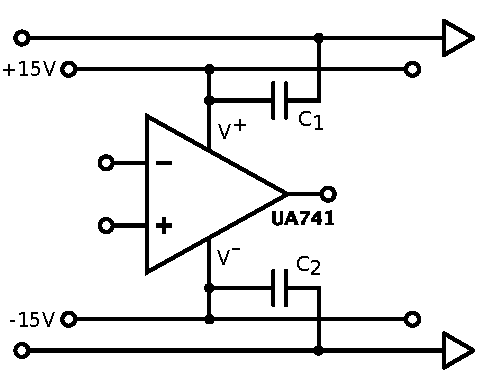
\includegraphics[width=6cm]{../E01/latex/alimentazione.pdf}}
 \caption{Grafico dell'alimentazione dell'OPAMP. La tensione di alimentazione è fornita con il generatore di tensione costante, mentre le capacità sono $C_1=(0.112 \pm 0.001)$ \si{\micro\farad} $C_2=(0.095\pm0.001)$ \si{\micro\farad}. Per maggiore chiarezza negli schemi circuitali, questa configurazione sarà nascosta negli schemi successivi, ma comunque presente sulla breadboard.}
 \label{gr:costante}
\end{figure}

Inoltre, al fine di evitare problemi di rumore durante l'alimentazione, abbiamo collegato l'alimentazione a due capacità come nello schema in Figura \ref{gr:costante}.

\section{Generatore di corrente}

In questo circuito abbiamo assemblato un generatore di corrente costante, cioè un dispositivo in grado di erogare una corrente costante ai capi di una resistenza (che definiremo \textit{resistenza di carico} $R_c$), indipendentemente dal valore di quest'ultima. Per valutare questa caratteristica abbiamo dunque utilizzato come $R_c=R_2$ una resistenza variabile di tipo \textit{trimmer}. Lo schema circuitale è in Figura \ref{gen_continua}.

\begin{wrapfigure}[21]{r}{0.55\textwidth}
  \begin{center}
    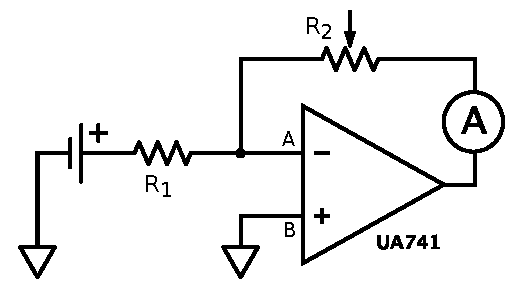
\includegraphics[width=0.40\textwidth]{../E01/latex/c1.pdf}
  \end{center}
  \caption{Schema del generatore di corrente costante. Come valori abbiamo utilizzato $R1=(3.85 \pm 0.01)$ \si{\kilo\ohm} e $V_{gen}=3.85$ \si{\volt}, mentre $R_2$ è variabile. Come amperometro è utilizzato il multimetro, mentre per alimentare l'OPAMP e come generatore di tensione costante in figura, abbiamo utillizzato il generatore Agilent E3631A.}
  \label{gen_continua}
\end{wrapfigure}

Risolviamo ora il circuito, considerando la tensione fornita dal generatore di tensione continua come $V_{gen}$ e la tensione in uscita dall'OPAMP come $V_{out}$. Dato che B si trova a potenziale di comune, per (\ref{eq:regola_V}) anche A sarà allo stesso potenziale, che considereremo nullo. Dunque varranno
\begin{equation}
V_{gen} - V_A = V_{gen} = I_1 R_1
\label{eq:gen_1}
\end{equation}
$$V_A-V_{out} = -V_{out} = I_2 R_2$$
Per (\ref{eq:regola_I}) e la legge di Kirkhhoff sui nodi, avremo invece che la corrente passante per la resistenza di carico è uguale alla corrente di (\ref{eq:gen_1}). Dunque $I=I_1=I_2$.

Otteniamo dunque che la tensione di output si modificherà, ad opera dell'OPAMP, in modo da far passare sempre lo stesso valore di corrente attraverso $R_2$; ciò avviene per il fenomeno di retroazione negativa, che ci permette di controllare la tensione di output tramite la resistenza di feedback, che in questo caso è $R_2$, e di ottenere dunque una corrente costante passante per il circuito di feedback. Imponendo l'uguaglianza della corrente possiamo inoltre trovare il valore della tensione di uscita

$$V_{out}=-\frac{R_2}{R_1} V_{gen}$$

Durante l'esperienza abbiamo però deciso di misurare la corrente passante per la resistenza piuttosto che la tensione di uscita, ponendo un amperometro fra l'uscita dell'OPAMP e la resistenza di carico $R_2$. Come valore di corrente abbiamo scelto $1$ \si{\milli\ampere}, discostandoci dalla corrente massima in cui l'amplificatore operazionale potrebbe non comportarsi più in maniera ideale ($10/20$ \si{\milli\ampere}); e avendo a disposizione una resistenza $R_1=(3.85 \pm 0.01)$ \si{\kilo\ohm}, per (\ref{eq:gen_1}), abbiamo utilizzato una tensione continua di $3.85$ \si{\volt}. Di seguito proponiamo alcuni valori sperimentali che confermano la capacità del circuito da noi creato di fornire alla resistenza di carico una corrente costante di $1$ \si{\milli\ampere}.

\begin{center}
\begin{tabular}{c|c|c|c|c|c|c|c|c}
Resistenza variabile [\si{\ohm}] & 0.54 & 35.1 & 412 & 1021 & 1996 & 3068 & 4170 & 4719 \\ 
\hline 
Corrente nel carico [\si{\milli\ampere}] & 1.002 & 1.002 & 1.002 & 1.002 & 1.002 & 1.002 & 1.002 & 1.002 \\ 
\end{tabular}
\end{center}

Gli errori sulla tabella sono uguali, cioè unitari sull'ultima cifra del valore, sia per le resistenza che per le correnti.

\section{Sommatore Pesato}

\subsection{Circuito}

Valutiamo ora il sommatore pesato, cioè un circuito che dati alcuni segnali in ingresso (due nel nostro caso) li somma con relativi pesi dati dal rapporto fra la resistenza di feedback ($R_f$) e quella a loro associata ($R_1$ e $R_2$). Lo schema circuitale è in Figura \ref{sommatore_pesato}.

\begin{wrapfigure}[21]{l}{0.55\textwidth}
  \begin{center}
    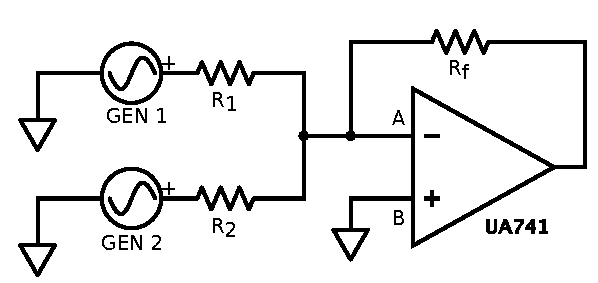
\includegraphics[width=0.40\textwidth]{../E01/latex/c2.pdf}
  \end{center}
  \caption{Schema del sommatore pesato. Come valori abbiamo utilizzato $R_f=(99.7 \pm 0.1)$ \si{\kilo\ohm}, $R_1=(99.9 \pm 0.1)$ \si{\kilo\ohm} e $R_2=(49.8 \pm 0.1)$ \si{\kilo\ohm}, dove per $R_2$ è stato necessario utilizzare un parallelo di due resistenza da $100$ \si{\kilo\ohm}. Come GEN 1 abbiamo utilizzato l'oscilloscopio, mentre per GEN 2 il generatore di forme d'onda. Infine, per valutare la tensione in uscita abbiamo utilizzato l'oscilloscopio.}
  \label{sommatore_pesato}
\end{wrapfigure}

Per risolvere il circuito consideriamo, definendo le tensioni dei generatori 1 e 2 rispettivamente $V_1$ e $V_2$, le seguenti equazioni derivanti dalle leggi di Kirkhhoff e dalla (\ref{eq:regola_I})
$$V_1 - V_A =I_1 R_1 \qquad V_2 - V_A =I_2 R_2$$
$$V_A - V_{out} =(I_1+I_2) R_f$$
Per (\ref{eq:regola_V}) vale inoltre che $V_A=V_B=0$; dunque otteniamo, sostituendo le correnti nell'ultima equazione sopra
$$V_{out}=-R_f \left( \frac{V_1}{R_1}+\frac{V_2}{R_2}\right)$$

Si può dunque definire un peso relativo $\phi_i$ ad ogni segnale dato dal rapporto fra $R_f$ ed $R_{i}$ (con $i=1,2$) e scrivere una formula del tipo
$$V_{out}=-\sum^{2}_{i=1} \frac{R_f}{R_{i}}V_{i}=-\sum^{2}_{i=1} \phi_i V_{i}$$

Durante l'esperienza abbiamo optato per valori semplici dei rapporti fra le resistenze, utilizzando i seguenti valori: $R_f=R_1=100 k\Omega$ e $R_2=50 k\Omega$. Si ottengono dunque $\phi_1=1$ e $\phi_2=2$.

\subsection{Grafici}

Presentiamo ora i grafici di alcune forme d'onda in uscita.

$$$$

\begin{figure}[ht]
 \centering
   {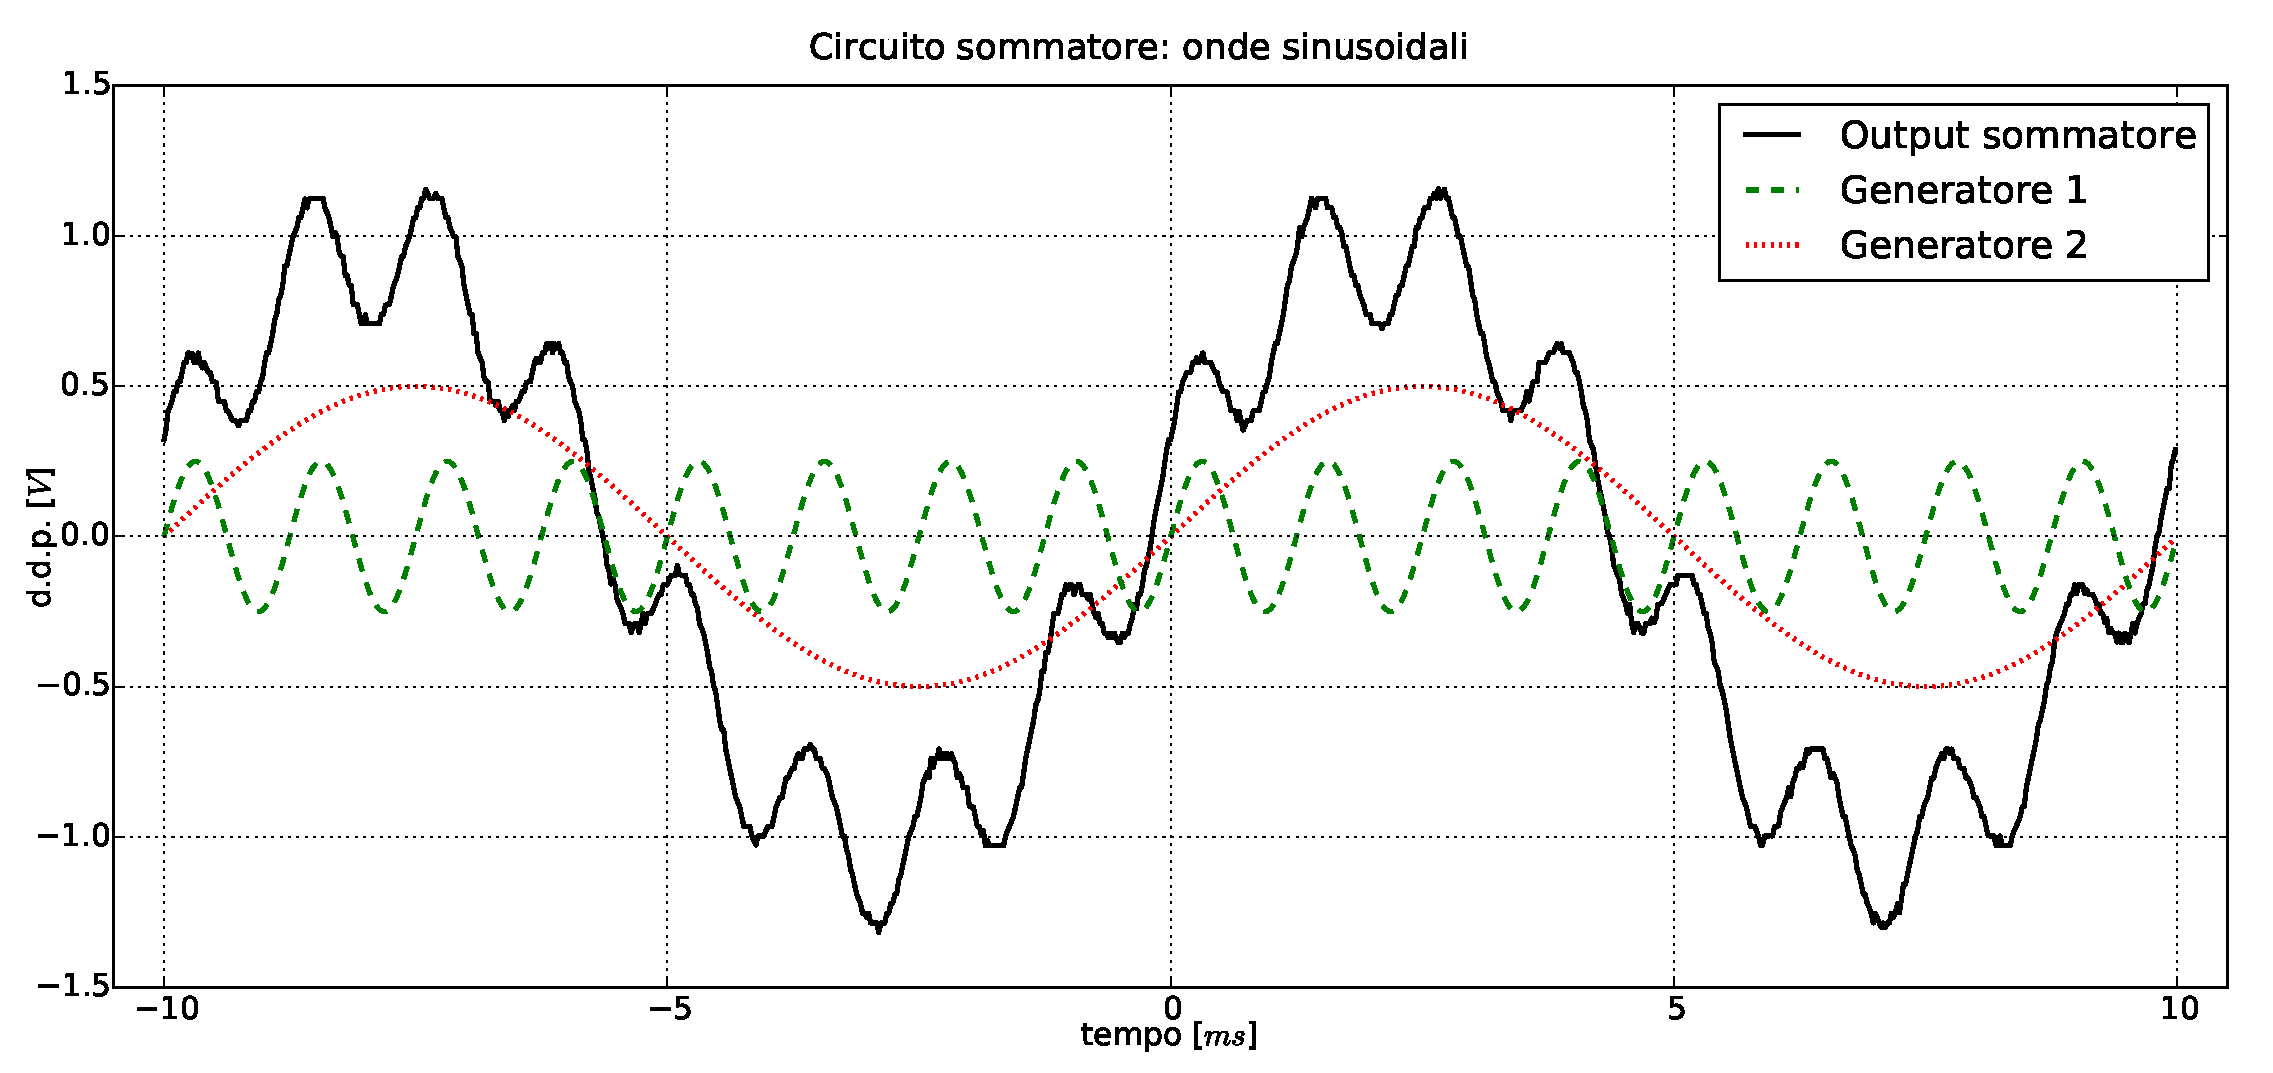
\includegraphics[width=16.5cm]{../E01/latex/sinsin.pdf}}
 \caption{Grafico della tensione di uscita. Il generatore 1 (generatore dell'oscilloscopio) crea un'onda sinusoidale di $\nu=800$ \si{\hertz} e $V^1_{pp}=500$ \si{\milli\volt}; il generatore 2 (generatore di forme d'onda) crea invece un'onda sinusoidale di $\nu=100$ \si{\hertz} e $V^2_{pp}=1000$ \si{\milli\volt}. Notiamo inoltre che l'ampiezza massima è pari a $\phi_1 V^1_{pp}+\phi_2 V^2_{pp}=2500$ \si{\milli\volt}.}
 \label{gr:onde1}
\end{figure}

$$$$

\begin{figure}[ht]
 \centering
   {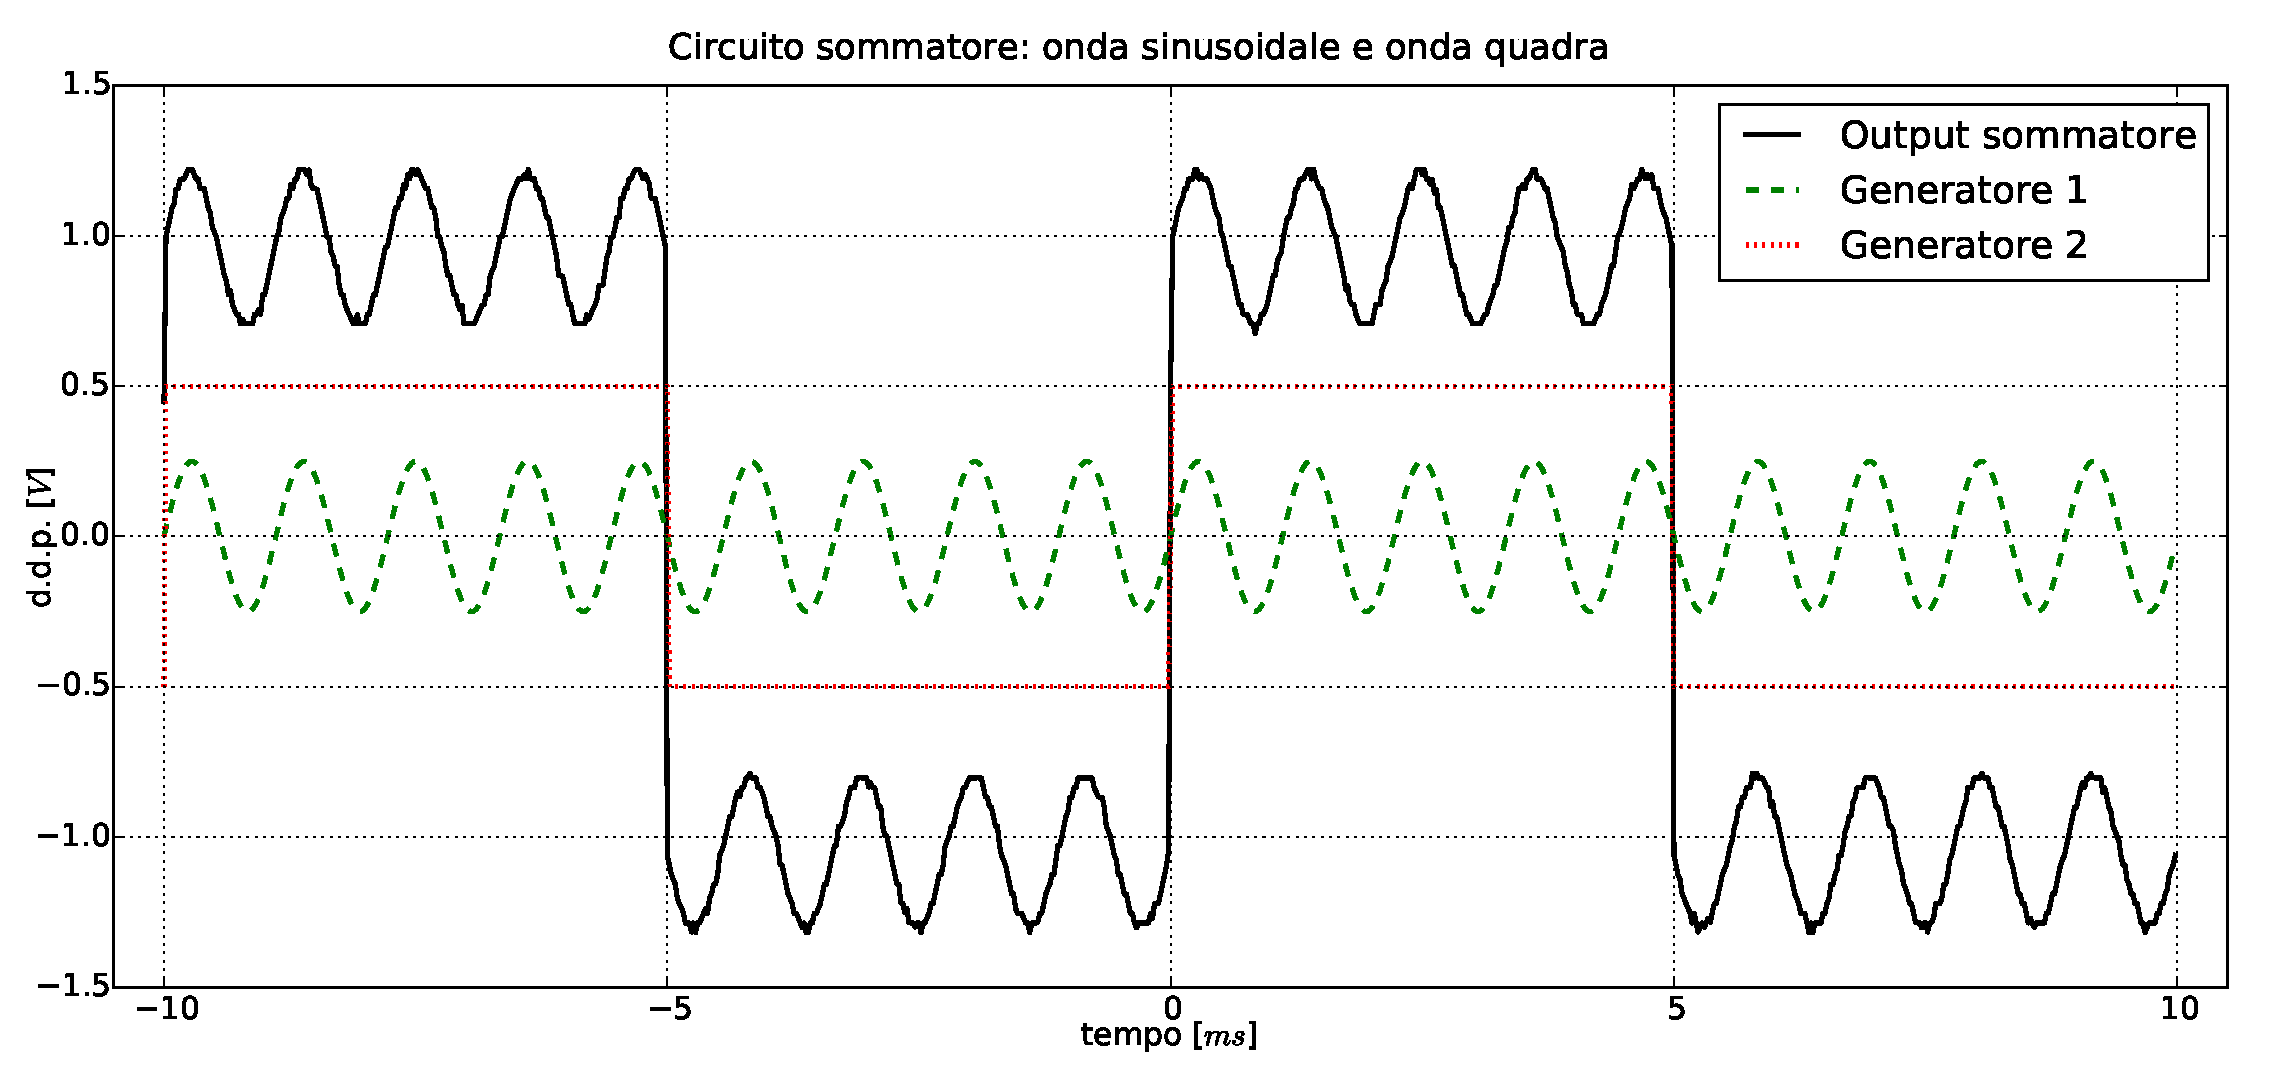
\includegraphics[width=16.5cm]{../E01/latex/sinquad.pdf}}
 \caption{Grafico della tensione di uscita. Il generatore 1 (generatore dell'oscilloscopio) crea un'onda sinusoidale di $\nu=900$ \si{\hertz} e $V^1_{pp}=500$ \si{\milli\volt}; il generatore 2 (generatore di forme d'onda) crea invece un'onda quadra di $\nu=100$ \si{\hertz} e $V^2_{pp}=1000$ \si{\milli\volt}. Notiamo inoltre che anche in questo caso l'ampiezza massima è pari a $\phi_1 V^1_{pp}+\phi_2 V^2_{pp}=2500$ \si{\milli\volt}.}
 \label{gr:onde2}
\end{figure}

\subsection{Battimenti}

Utilizzando due forme d'onda sinusoidali con il sommatore, abbiamo potuto il battimento, fenomeno che si verifica quando la differenza fra le frequenze delle onde in ingresso è sufficientemente bassa.

Con due onde abbiamo che:
$$V_{out}=\phi_1 A_1 \sin [2 \pi \nu_1 t + \theta_1] + \phi_2 A_2 \sin [2 \pi \nu_2 t + \theta_2]$$

Supponiamo che $A=\phi_1 A_1=\phi_2 A_2$, come nel caso del grafico sotto riportato. Utilizzando le formule di prostaferesi otteniamo che

$$V_{out}=2A \sin \left[4 \pi (\nu_1 + \nu_2) t + \frac{\theta_1+\theta_2}{2}\right] \cos \left[4 \pi (\nu_1 - \nu_2)t + \frac{\theta 1-\theta_2}{2}\right]$$


\begin{figure}[ht]
 \centering
   {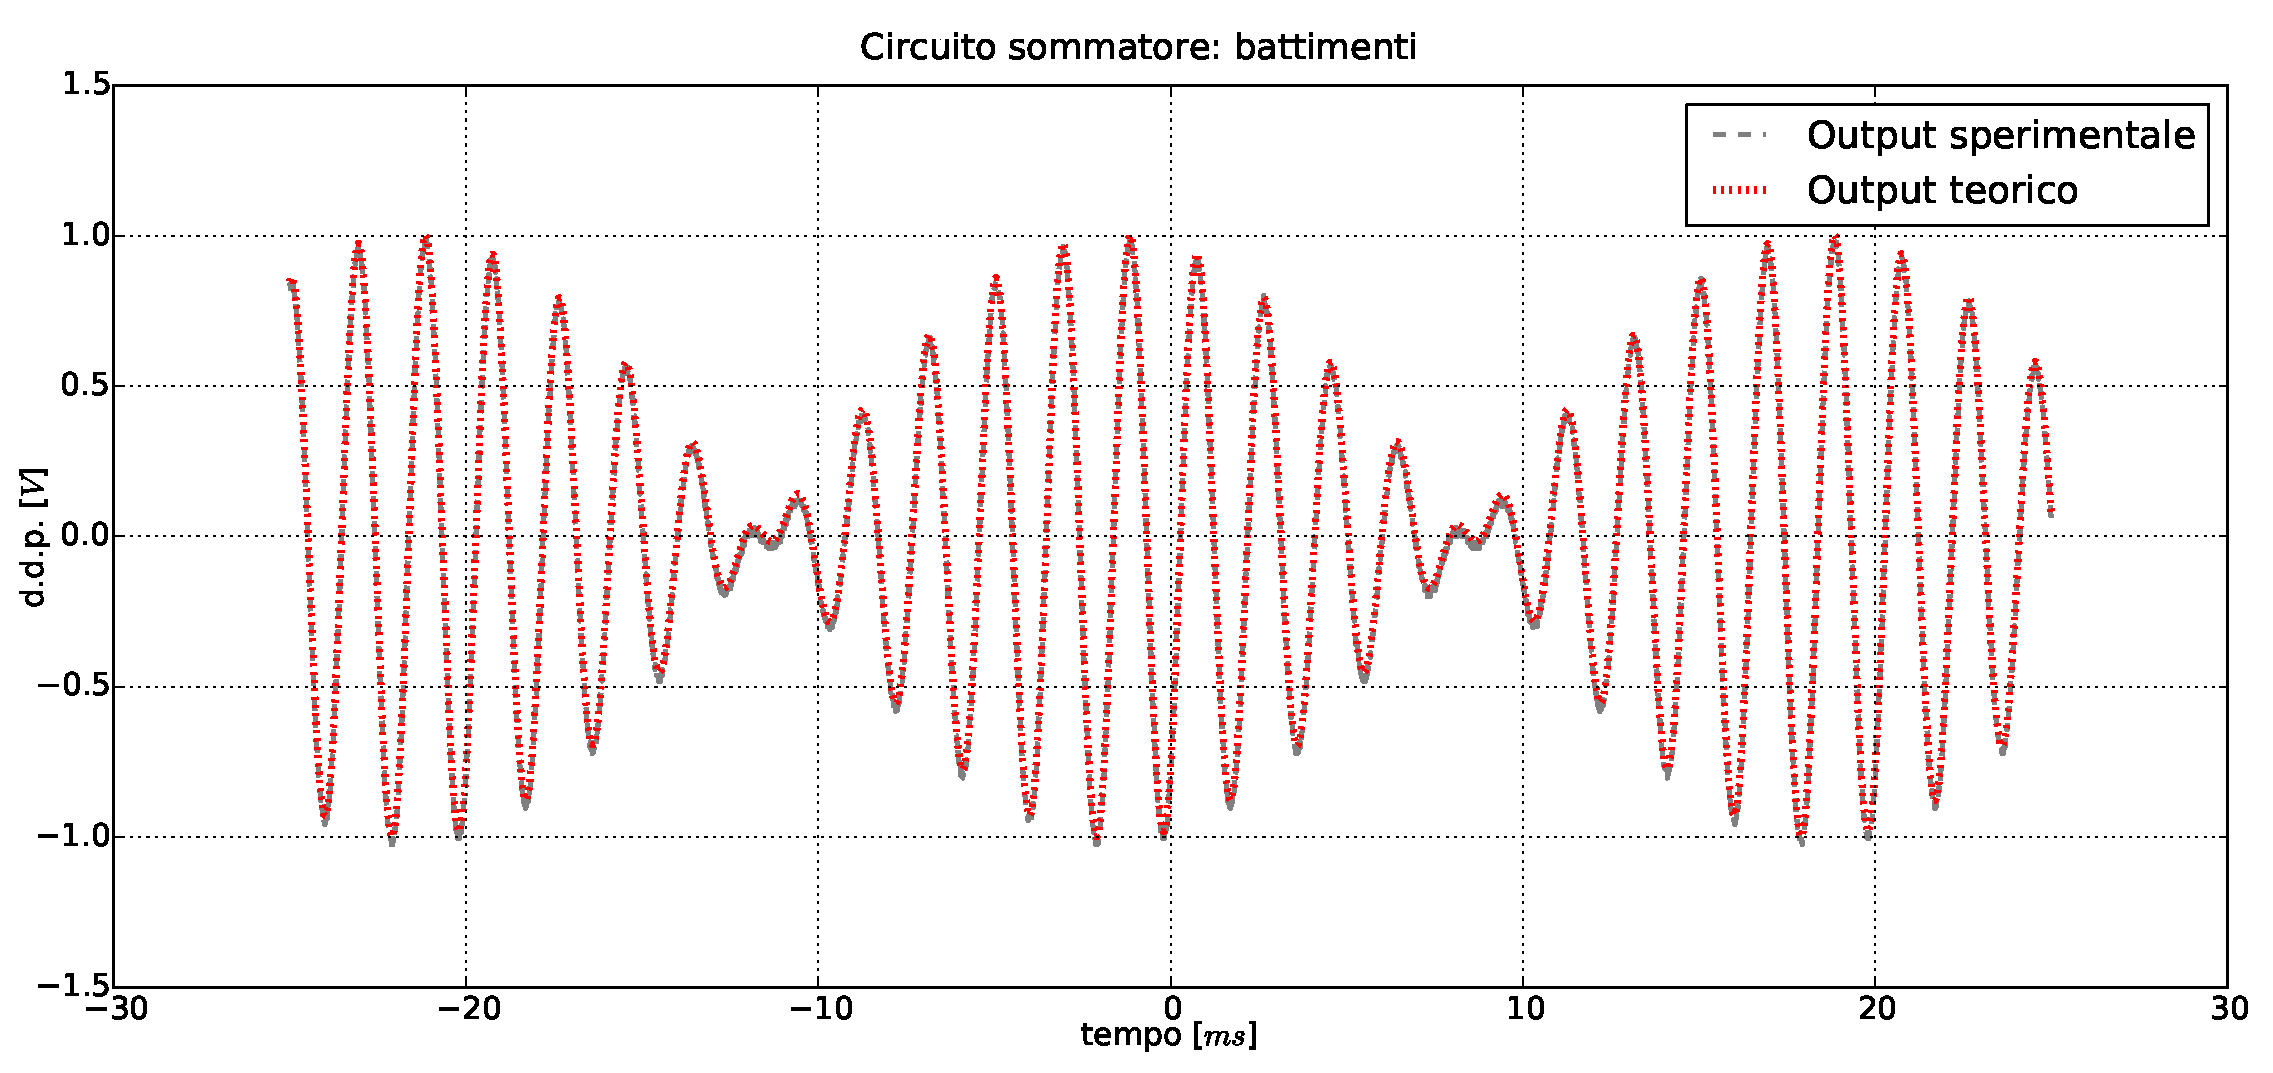
\includegraphics[width=17.5cm]{../E01/latex/battimenti_ideali.pdf}}
 \caption{Grafico della tensione di uscita. Il generatore 1 (generatore dell'oscilloscopio) crea un'onda sinusoidale di $\nu=900$ \si{\hertz} e $V^1_{pp}=500$ \si{\milli\volt}; il generatore 2 (generatore di forme d'onda) crea invece un'onda quadra di $\nu=100$ \si{\hertz} e $V^2_{pp}=1000$ \si{\milli\volt}. Notiamo inoltre che anche in questo caso l'ampiezza massima è pari a $\phi_1 V^1_{pp}+\phi_2 V^2_{pp}=2500$ \si{\milli\volt}.}
 \label{gr:battimenti}
\end{figure}
\section{24.09.2014 - Amplificatori operazionali reali}

Scopo di questa esperienza è quello di studiare un amplificatore operazionale $\mu$A741.
Ne analizzeremo l'offset e le correnti di polarizzazione (\textit{bias currents}) cercando di stimarne un valore, tramite circuiti progettati ad hoc.
Premettiamo che il circuito di alimentazione è lo stesso utilizzato nella precedente esperienza e dunque non ripeteremo le considerazioni e gli schemi circuitali già proposti.
Inoltre ricordiamo che la circuiteria di alimentazione sugli schemi è stata nascosta per facilitarne la comprensione.

\subsection{Strumenti e materiali}

\begin{itemize} [noitemsep]
\item Generatore di tensione continua Agilent E3631A (max $\pm \, \SI{25}{\volt}$ o $\pm \, \SI{6}{\volt}$);
\item Multimetro Agilent 34410A a sei cifre e mezza;
\item Un amplificatore operazionale $\mu$A741;
\item Resistenze e capacità di vari valori;
\item un trimmer a un giro da \SI{5}{\kilo\ohm} e uno da \SI{10}{\kilo\ohm};
\item un trimmer multigiro da \SI{10}{\kilo\ohm};
\item Breadboard e cablaggi vari.
\end{itemize}

\subsection{Stima e correzione dell'offset}
\label{par2:offset}

In questa prima parte dell'esperienza tratteremo il problema dell'offset. In un amplificatore ideale sappiamo che quando sia ingresso invertente che ingresso non invertente sono collegati a comune il segnale in uscita è nullo. Ciò è dovuto alla perfetta simmetria interna dell'op-amp. Ovviamente nel mondo reale non è possibile realizzare tale fatto in quanto non si riescono a costruire transistor BJT con specifiche identiche. 

\subsubsection{Configurazione senza retroazione}

Quando colleghiamo entrambi gli ingressi a comune l'op-amp vede all'ingresso una differenza di potenziale (ovviamente, fra gli ingressi non c'è, in quanto collegati entrambi a comune) la quale viene amplificata dal guadagno a maglia aperta: come $V_{out}$ avremo dunque un valore diverso da zero. Nel nostro caso l'op-amp andava in saturazione negativa (\SI{-14.3}{\volt}). Ricordando il funzionamento di un amplificatore operazionale, possiamo dire che il circuito si comporta come se la tensione all'ingresso invertente fosse maggiore di quella all'ingresso non invertente. Inoltre il valore $V_{out}$ è diverso da \SI{-15}{\volt} utilizzati come alimentazione in quanto il valore di tensione massimo $|V_{out}|$ è leggermente inferiore a $|V^-|$. In Figura(\ref{cir:open_loop}) è riportato lo schema del circuito utilizzato.

\begin{figure}[ht]
        \centering
        \begin{subfigure}[b]{0.35\textwidth}
                 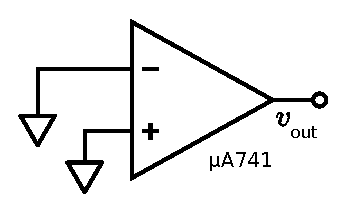
\includegraphics[width=0.70\textwidth]{../E02/latex/open_loop.pdf}
                \caption{Circuito a maglia aperta}
                \label{cir:open_loop}
        \end{subfigure}%
    \quad
        \begin{subfigure}[b]{0.35\textwidth}
               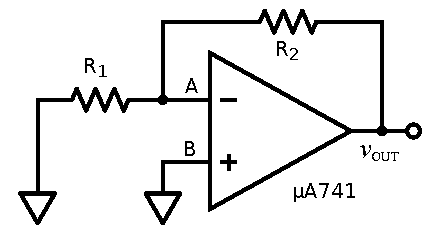
\includegraphics[width=0.70\textwidth]{../E02/latex/inv.pdf}
                \caption{Circuito amplificatore}
                \label{cir:inv}
        \end{subfigure}
     
\end{figure}

Con il circuito in Figura (\ref{cir:open_loop}) non possiamo quindi ricavare una stima del valore di offset. Per fare ciò dobbiamo ricorrere a un circuito amplificatore come quello in Figura(\ref{cir:inv}) (invertente o non invertente), che ci permetta di controllare il guadagno.

\subsubsection{Configurazione con retroazione}

Trattiamo per primo il caso \textbf{invertente}. Assumiamo nel punto A la presenza di un generatore di tensione $V_A=V_{off}$ e consideriamo $V_B=0$. Vale allora che, uguagliando le correnti

$$\frac{V_{off}}{R_1} + \frac{V_{off}-V_{out}}{R_2} = 0$$

da cui si ricava che
$$V_{out}=\left(1+\frac{R_2}{R_1}\right) V_{off}$$

Analogamente si tratta il caso \textbf{non invertente}. Per far ciò immaginiamo nel punto B un generatore di tensione $V_B=-V_{off}$ . Si ottiene lo stesso risultato ricavato per il caso \textbf{invertente}.

%I valori nominali delle componenti circuitali utilizzate sono: $R_1=\SI{120}{\ohm}$ e $R_2=\SI{10/100}{\kilo\ohm}$.

Riportiamo nella seguente tabella i valori di offset calcolati, definendo il guadagno = $1+\frac{R_2}{R_1}$. 

\begin{center}
\begin{savenotes}
\begin{tabular}{c|c|c|c|c|c|c}
$R_1[\si{\ohm}]$ & $R_2[\si{\kilo\ohm}]$ & Gain &$V_{out} [\si{\milli\volt}]$ & $V_{off}$ [\si{\milli\volt}]\\ 
\hline 
$119.8\pm0.1$ & $9.911\pm0.001$ & $83.73\pm0.07$&  $-103.5 \pm 0.5$ & $-1.23 \pm0.01$\\
\hline
$119.8\pm0.1$ & $99.35\pm0.01$ & $830.3\pm0.7$ &$ -1025 \pm 2$ & $-1.2 \pm0.1$\\

\end{tabular}
\end{savenotes}
\end{center}

\begin{wrapfigure}[17]{l}{0.55\textwidth}
  \begin{center}
    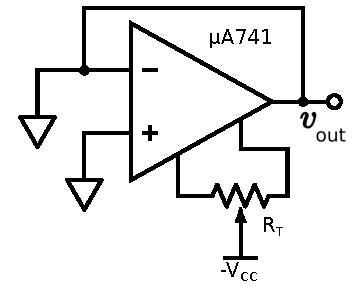
\includegraphics[width=0.280\textwidth]{../E02/latex/trimmer_correction.pdf}
  \end{center}
  \caption{Circuito a guadagno unitario, con trimmer sui piedini 1 e 5 dell'OPAMP per compensare l'offset.}
  \label{cir2:trimmer}
\end{wrapfigure}

%Come sappiamo la tensione di offset non è però l'unico problema che incontriamo quando usiamo op-amp reali. Infatti ingresso invertente e non invertente sono collegati alle basi di transistor e, ovviamente, per polarizzarli serve una corrente di base. Gli effetti di tale corrente si sommeranno dunque a quelli dovuti all'offset. Tale argomento sarà comunque trattato approfonditamente nella sezione successiva. 

Per risolvere il problema dell'offset possiamo servirci di una resistenza variabile ($trimmer$) che posizioneremo tra i piedini 1 e 5 dell'op-amp, collegandola a $V^-$. Regolando tale resistenza andremo a generare una contro tensione che bilancerà l'offset. Il circuito utilizzato per verificare il bilanciamento dell'offset è quello in Figura \ref{cir2:trimmer}.

Durante l'esperienza abbiamo utilizzato un trimmer multigiro da \SI{10}{\kilo\ohm}, con il quale abbiamo raggiunto la tensione $V_{out}\simeq 0\si{\volt}$. Come verifica abbiamo misurato la tensione $V_{out}$ a maglia aperta, ottenendo il valore $V_{out}=1.3\pm0.2$. Ricordando che il guadagno $A_{ol}$ è di 100-120dB, si nota il buon bilanciamento della tensione di offset.

\begin{wrapfigure}[17]{r}{0.55\textwidth}
  \begin{center}
    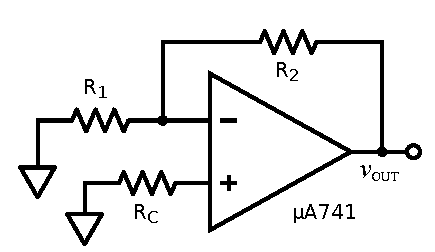
\includegraphics[width=0.280\textwidth]{../E02/latex/current_correction.pdf}
  \end{center}
  \caption{Circuito utilizzato per la stima di $V_{off}$ con la correzione sulle correnti data da $R_C$.}
  \label{cir2:current_correction}
\end{wrapfigure}

Come sappiamo attraverso gli ingressi invertente e non invertente dell'amplificatore operazionale reale scorrono delle correnti, dette di bias. Queste, per quanto piccole (\si{\nano\ampere}), hanno comunque un contributo sull'offset totale. Per minimizzare il loro impatto sul valore della tensione di offset abbiamo inserito fra l'ingresso non invertente e comune una resistenza di compensazione $R_C$ tale da annullare il contributo delle correnti di offset sulla tensione di uscita.

Il contributo alla tensione di uscita data dalle correnti di polarizzazione, supponendo già l'offset compensato, è

\begin{equation}
V_{out}^{C} = \left( 1+\frac{R_2}{R_1} \right)\left[ \frac{I_{b^-}R_2}{\frac{R_1+R_2}{R_1}} - I_{b^+} R_C\right]
\label{eq2:Vout_currents}
\end{equation}

dalla quale, se $|I_{b^+}|\simeq|I_{b^-}|$ e $V_{out}^{C}=0$, banalmente otteniamo

$$R_C=\frac{1}{\frac{1}{R_1} + \frac{1}{R_2}} $$



Riportiamo nella seguente tabella i nuovi valori in questa nuova configurazione (circuito in Figura \ref{cir2:current_correction}):

\begin{center}
\begin{tabular}{c|c|c|c|c|c|c}
$R_C [\si{\ohm}]$& $R_1[\si{\ohm}]$ & $R_2[\si{\kilo\ohm}]$ & Gain & $V_{out}' [\si{\milli\volt}]$ & $V_{off}' [\si{\milli\volt}]$ & $|V_{off}-V_{off}'|[\si{\milli\volt}]$ \\ 
\hline 
$119.4\pm0.1$ & $119.8\pm0.1$ & $9.911\pm0.001$  & $83.73 \pm 0.07$ & $-105.5 \pm 0.5$ & $-1.26 \pm0.01$ & $0.02\pm0.01$ \\
\hline
$119.4\pm0.1$ & $119.8\pm0.1$ & $99.35\pm0.01$  & $830.3\pm0.7$ &$ -1038 \pm 5$ & $-1.2 \pm 0.1$ & $\approx 0$\\
\end{tabular}
\end{center}

Notiamo che le differenze fra i valori della tensione di offset con e senza $R_C$ sono compatibili con il rumore ambientale (qualche decina di \si{\micro\volt} di ampiezza). Se osserviamo la tensione $V_{out}$ nei casi con e senza resistenza $R_C$, notiamo una differenza di circa $13\si{\milli\volt}$. Nel successivo paragrafo stimeremo una corrente di bias di $37\si{\nano\ampere}$. Possiamo dunque osservare che la caduta di potenziale su tale resistenza dovuta alla corrente di polarizzazione è $\Delta V \simeq 3 \si{\milli\volt}$. Tale valore è circa 4 volte più piccolo della differenza delle tensioni in uscita misurate. Nella stima dell'offset abbiamo dunque il contributo delle correnti di bias ma essendo dello stesso ordine di grandezza del rumore ambientale (o addirittura inferiore) non possiamo valutarne quantitativamente gli effetti. 

\subsection{Correnti di polarizzazione}

\begin{wrapfigure}[12]{r}{0.55\textwidth}
  \begin{center}
    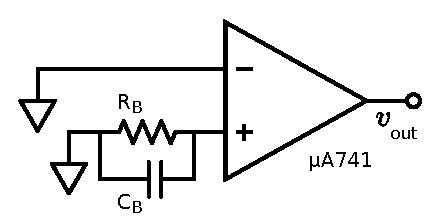
\includegraphics[width=0.30\textwidth]{../E02/latex/direct_measure.pdf}
  \end{center}
  \caption{Schema del circuito non retro-azionato utilizzato per stimare la corrente di polarizzazione. La resistenza utilizzata è $R_B=10.36\pm0.01$\si{\mega\ohm}; la capacità $C_B=102 \pm 1$ \si{\nano\farad}.}
  \label{circuito:rel2_correnti_senzaretroazione}
\end{wrapfigure}


Nella seconda parte dell'esperienza abbiamo misurato le correnti di polarizzazione che scorrono nei due ingressi. Ricordiamo che la tensione di offset è già stata compensata dall'esterno con l'utilizzo di un \textbf{trimmer}. 

\subsubsection{Misura diretta}





Come primo approccio abbiamo tentato una misura diretta della corrente $I_{b^+}$.
Abbiamo utilizzato una resistenza molto grande (10\si{\mega\ohm}) prima dell'ingresso non invertente (analogamente si può fare con l'ingresso invertente) e abbiamo misurato la tensione ai suoi capi. La legge di ohm ci assicura che $I_{b^+}=\frac{V}{R}$. A causa del rumore di fondo però il valore misurato non era stabile. Si è dunque pensato di aggiungere in parallelo alla resistenza un condensatore, così da stabilizzare la tensione.




%Per far ciò, dato che attendevamo una corrente dell'ordine dei \si{\nano\ampere}, abbiamo utilizzato una resistenza molto grande in modo da poter leggere il valore della tensione su una scala accettabile per il multimetro.

%Durante la procedura abbiamo però notato che, a causa di rumori ambientali, il valore di tensione sul multimetro fluttuava sulla prima cifra, rendendo nostra misurazione ovviamente non quantitativa (al massimo poteva stimarci l'ordine di grandezza della corrente). Per ovviare, abbiamo inserito in parallelo alla resistenza un condensatore che caricandosi si portava alla stessa ddp dei capi della resistenza. In questo modo abbiamo potuto ottenere un valore meno fluttuante, che si attestava a $V=(-80 \pm 2)$ \si{\milli\volt}, cioè $I_{b^+}=(7.7 \pm 0.2)$ \si{\nano\ampere}.

Il valore che siamo riusciti a stimare con la stabilizzazione con condensatore è $V=(-80 \pm 2) \si{\milli\volt} \Rightarrow I_{b^+}=(7.7 \pm 0.2)$ \si{\nano\ampere}.


%Con questo metodo semplice abbiamo potuto ottenere una prima stima del valore della corrente. Di contro bisogno considerare che il rumore non permette di avere una stima qualitativa ed inoltre la resistenza, scaldandosi, modifica il suo valore e potrebbe portare ad un errore sulla misura. Successivamente progetteremo dunque un circuito che, sfruttando l'amplificazione data dall'amplificatore operazionale, minimizzerà questi errori.

I difetti di tale metodo di misura sono molteplici. Anzitutto la resistenza si scalda e ciò produce un aumento della resistenza stessa ($\approx 5 ppm/^{\circ}C$).





\subsubsection*{Misura di $I_{b^-}$}

\begin{wrapfigure}[15]{l}{0.55\textwidth}
  \begin{center}
    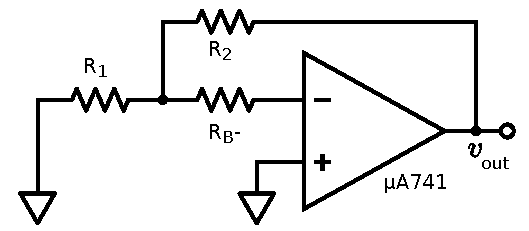
\includegraphics[width=0.30\textwidth]{../E02/latex/inv_current.pdf}
  \end{center}
  \caption{Schema del circuito retro-azionato utilizzato per stimare la corrente di polarizzazione $I_{b^-}$. Le resistenze utilizzate sono $R_1=(98.9\pm0.1)$ \si{\ohm}, $R_2=(99.4\pm0.1)$ \si{\kilo\ohm} e $R_B=(99.4\pm0.1)$ \si{\kilo\ohm}.}
  \label{circuito:rel2_correnti_retroazione_inv}
\end{wrapfigure}

Come secondo approccio abbiamo dunque provato una misura indiretta della corrente $I_{b^-}$. Per fare ciò abbiamo utilizzato il circuito in Fig. \ref{circuito:rel2_correnti_retroazione_inv}. Ricordiamo che la tensione di offset è già stata compensata esternamente.

%Chiamiamo $V_{-}$ la tensione al capo di $R_B$ collegato all'OPAMP e $V^*$ quello opposto, vale in quel punto la legge di Kirchhoff sui nodi
Chiamiamo $V_{inv}$ la tensione all'ingresso invertente e $V_{nodo}$ la tensione nel nodo in cui sono collegate tra loro $R_B$,$R_1$ e $R_2$. Basta ora risovere il seguente sistema 


$\begin{cases} \frac{V_{nodo} - V_{in}}{R_1} + \frac{V_{nodo}-V_{out}}{R_2} + \frac{V_{nodo}-V_{inv}}{R_B}=0 \\ V_{in}=V_{inv}=0  \\I_{b^-} = \frac{V_{nodo}}{R_B} \end{cases} $

Da cui segue dopo alcuni calcoli algebrici

%$$\frac{V_{nodo} - V_{in}}{R_1} + \frac{V_{nodo}-V_{out}}{R_2} + \frac{V_{nodo}-V_{inv}}{R_B}=0$$

%Per la struttura del circuito e la compensazione dell'offset è immediato vedere che $V_{in}=V_{inv}=0$ e, se definiamo la corrente $I_{b^-} = \frac{V_{nodo}}{R_B}$):

$$I_{b^-}=\frac{V_{out}}{R_2 R_B}\frac{1}{\frac{1}{R_1}+\frac{1}{R_2}+\frac{1}{R_B}}$$

Le resistenze sono state dimensionate in modo da ottenere tensioni $V_{out}$ dell'ordine del Volt.
La misura di tensione di uscita è di $(3.89\pm0.02)\si{\volt} \Rightarrow I_{b^-} = (38 \pm 5)$ \si{\nano\ampere}.

\subsubsection*{Misura di $I_{b^+}$}

\begin{wrapfigure}[17]{r}{0.55\textwidth}
  \begin{center}
    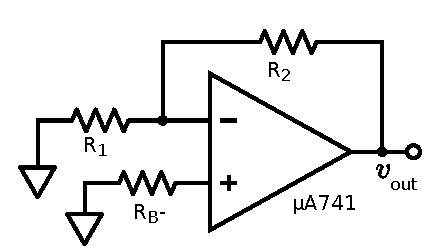
\includegraphics[width=0.25\textwidth]{../E02/latex/ninv_current.pdf}
  \end{center}
  \caption{Schema del circuito retro-azionato utilizzato per stimare la corrente di polarizzazione $I_{b^+}$. Le resistenze utilizzate sono le medesime del circuito precedente in Figura \ref{circuito:rel2_correnti_retroazione_inv}.}
  \label{circuito:rel2_correnti_retroazione_noninv}
\end{wrapfigure}

%Similmente a quanto visto per la configurazione prima, troviamo che, data la legge di Kirchhoff (con $V^*$ la tensione all'ingresso non invertente, che per quanto detto sopra è uguale a quella all'ingresso invertente)

In questo secondo caso riportato in Fig. \ref{circuito:rel2_correnti_retroazione_noninv} chiamiamo $V_{ninv}$ la tensione all'ingresso non invertente.


$\begin{cases}\frac{V_{ninv} - V_{in}}{R_1} + \frac{V_{ninv}-V_{out}}{R_2}=0 \\ I_{b^+}=\frac{V_{ninv}}{R_B}\\ V_{in}=0 \end{cases}$

Risolvendo il sistema otteniamo


\begin{equation}
I_{b^+}=\frac{V_{out}}{R_2 R_B}\frac{1}{\frac{1}{R_1}+\frac{1}{R_2}}
\label{eq2:corrente_noninv}
\end{equation}

Anche in questo caso le resistenze sono state dimensionatein modo da ottenere un $V_{out}$ dell'ordine dei Volt. La misura di tensione di uscita è di $-(3.72 \pm 0.02) \si{\volt} \Rightarrow I_{b^+} = - (37.2 \pm 0.2)$ \si{\nano\ampere}

Ricordiamo che il segno della corrente dipende dalla convenzione scelta. Abbiamo deciso di assumere nei calcoli segno positivo per correnti entranti e segno negativo per correnti uscenti. La corrente $I_{b^-}$ sarà dunque entrante nell'ingresso inverntente mentre $I_{b^+}$ sarà uscente dall'ingresso invertente.

%\footnote{ La negatività della corrente è intesa rispetto all'ingresso non invertente, ed è quindi uscente rispetto a tale ingresso. Al contrario, nel paragrafo precedente, la corrente è intesa entrante nel punto di $V^*$, e quindi è entrante rispetto all'ingresso invertente.}.

\subsubsection*{Calcolo di $I_{b^+}$ data $I_{b^-}$}

Proviamo a calcolare $I_{b^+}$ utilizzando il valore di $I_{b^-}$ calcolato sopra e avvalendoci di Eq. (\ref{eq2:Vout_currents}). \'E triviale ricavare la seguente identità: 

$$I_{b^+} = \frac{R_1}{R_B(R_1+R_2)}(I_{b^-} R_2-V_{out})$$

Inserendo i valori numerici otteniamo $I_{b^+} = - (37.2 \pm 0.2)$ \si{\nano\ampere}, compatibile con il risultato precedente.


\subsubsection*{Cenni sul rumore termico}
Nel paragrafo sulla misura diretta della corrente di bias abbiamo ottenuto un valore non compatibile con quello stimato utilizzando la procedura indiretta. Proviamo a vedere se tale discrepanza può essere dovuta al rumore termico.
 
Consideriamo la larghezza di banda del multimetro $\Delta f = \SI{1}{\hertz}$ e siano $k_B = \SI{1.38e-23}{\joule\per\kelvin}$ la costante di Boltzmann, $T$ la temperatura assoluta e $R$ il valore della resistenza presa in considerazione

\begin{equation}
	V_{eff}^2 = 4 k_B T R \Delta f
\end{equation}

Inserendo i valori numerici e il valore di resistenza $R=\SI{10}{\mega\ohm}$ si ottiene che il rumore termico è 5 ordini di grandezza inferiore alla tensione misurata.

\begin{equation}
	V_{eff} = \sqrt{4 k_B T R \Delta f} \simeq 4 \times 10^{-7} \si{\volt}
\end{equation}






\subsection{Conclusioni}
In questa esperienza abbiamo studiato le caratteristiche di un OPAMP, misurandone tensione di offset e correnti di polarizzazione. La presenza dell'offset può essere bilanciata utilizzando semplicemente un trimmer collegato a 2 piedini dell'amplificatore operazionale. Così facendo possiamo creare una contro-tensione interna che bilancia automaticamente l'offset. Le correnti di polarizzazione, invece, possono essere bilanciate ottimizzando le impedenze in ingresso. Tuttavia, essendo dell'ordine dei \si{\nano\ampere}, giocano un ruolo solo nel caso si lavori con tensioni di pochi millivolt. Negli utilizzi più comuni (con tensioni dell'ordine dei Volt) possono essere trascurate.




%In questa esperienza abbiamo potuto osservare come gli OPAMP, sebbene siano dei circuiti abbastanza precisi, abbiano delle imperfezioni, date dalla loro composizione circuitale (sono presenti dei transistor BJT al loro interno).
%Le discrepanze tra il modello ideale e l'OPAMP reale sono date principalmente dallo sbilanciamento della risposta dello stesso ($V_{offset}$) e dalle correnti di polarizzazione (\textit{bias currents}).
%Per nostra fortuna spesso gli OPAMP presentano dei connettori predisposti a minimizzare la tensione di offset con circuiti di compensazione: nel nostro caso un trigger collegato ai piedini di offset e all'alimentazione negativa.
%Una volta bilanciato l'opamp, abbiamo misurato le correnti di polarizzazione e abbiamo potuto osservare che esse sono dell'ordine dei \si{\nano\ampere}, quindi trascurabili per gli utilizzi più comuni.

\end{document}
